\part{Vectors}
\frame{\partpage}

\begin{frame}{Vectors}
	\begin{columns}
		\begin{column}{0.48\textwidth}
			\pause A vector has \textbf{components}
			\pause 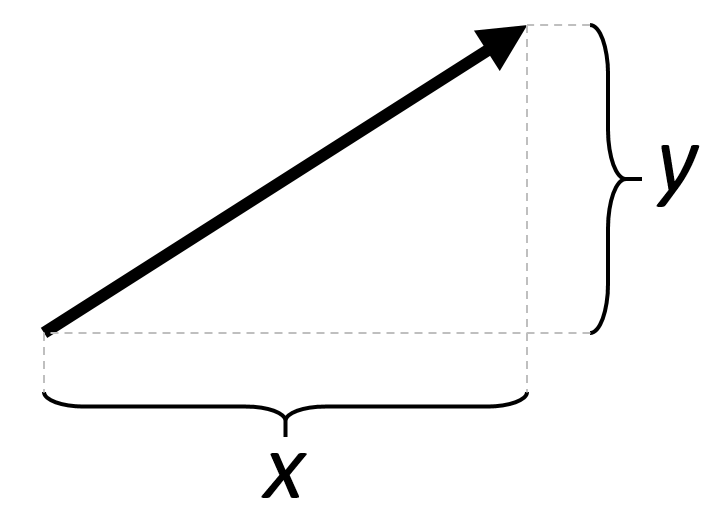
\includegraphics[width=\textwidth]{vector_components}
		\end{column}
		\begin{column}{0.48\textwidth}
			\pause A vector also has \textbf{direction} and \textbf{magnitude} (or \textbf{length})
			\pause 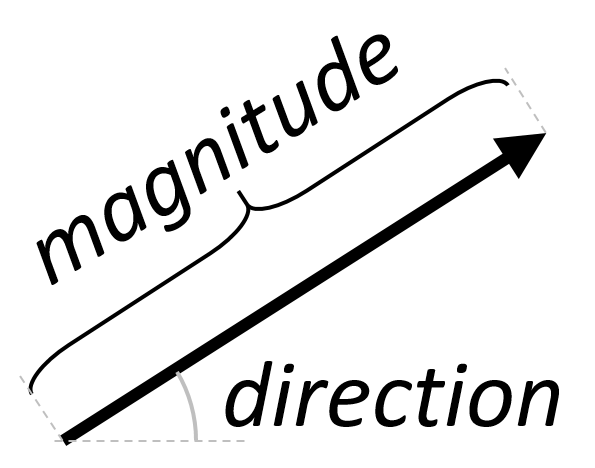
\includegraphics[width=\textwidth]{vector_polar}
		\end{column}
	\end{columns}
	\pause The \textbf{origin} is the point represented by the vector $(0, 0, \dots)$
\end{frame}

\begin{frame}{Radians}
	\begin{itemize}
		\pause\item We often measure angles in \textbf{radians}
		\pause\item $\pi = 3.14159\dots$ 
		\pause\item $\pi \text{ radians} = 180 \text{ degrees} = \text{half a circle}$ 
		\pause\item $\frac{\pi}{2} \text{ radians} = 90 \text{ degrees} = \text{right angle}$
		\pause\item Careful! Some things in OpenGL work in \textbf{degrees}, others in \textbf{radians}
			(just to confuse you...)
	\end{itemize}
\end{frame}

\begin{frame}{Right hand rule}
	\pause OpenGL uses a \textbf{right-handed coordinate system}
	\pause \begin{center}
		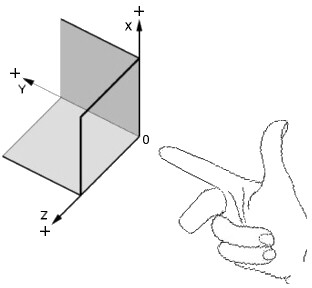
\includegraphics[width=0.3\textwidth]{RightHandRule}
	\end{center}
	\begin{itemize}
		\pause\item The \textbf{$x$-axis} points towards the \textbf{right-hand side} of the screen
		\pause\item The \textbf{$y$-axis} points towards the \textbf{top} of the screen
		\pause\item The \textbf{$z$-axis} points \textbf{out} of the screen
	\end{itemize}
\end{frame}

\begin{frame}{Homogeneous coordinates}
	\begin{itemize}
		\pause\item In 3D graphics, it is useful to represent a \textbf{point in 3D space} as a \textbf{4-dimensional vector}
		\pause\item The extra coordinate is called $w$
		\pause\item Simple explanation: $w$ should always equal $1$ for points in 3D space; having $w$ there makes certain calculations easier
			\begin{itemize}
				\pause\item (Actually, a point $(x,y,z)$ can be represented as a vector $(x \times w, y \times w, z \times w, w)$ for any $w \neq 0$)
			\end{itemize}
		\pause\item In homogeneous coordinates, the origin is $(0, 0, 0, 1)$ not $(0, 0, 0, 0)$!
	\end{itemize}
\end{frame}
